\let\negmedspace\undefined
\let\negthickspace\undefined
\documentclass[journal]{IEEEtran}
\usepackage[a5paper, margin=10mm, onecolumn]{geometry}
%\usepackage{lmodern} % Ensure lmodern is loaded for pdflatex
\usepackage{tfrupee} % Include tfrupee package

\setlength{\headheight}{1cm} % Set the height of the header box
\setlength{\headsep}{0mm}     % Set the distance between the header box and the top of the text

\usepackage{gvv-book}
\usepackage{gvv}
\usepackage{cite}
\usepackage{amsmath,amssymb,amsfonts,amsthm}
\usepackage{algorithmic}
\usepackage{graphicx}
\usepackage{textcomp}
\usepackage{xcolor}
\usepackage{txfonts}
\usepackage{listings}
\usepackage{enumitem}
\usepackage{mathtools}
\usepackage{gensymb}
\usepackage{comment}
\usepackage[breaklinks=true]{hyperref}
\usepackage{tkz-euclide}
\usepackage{listings}
\usepackage{pgfplots}
\pgfplotsset{compat=newest}
\def\inputGnumericTable{}
\usepackage[latin1]{inputenc}
\usepackage{color}
\usepackage{array}
\usepackage{longtable}
\usepackage{calc}
\usepackage{multirow}
\usepackage{hhline}
\usepackage{ifthen}
\usepackage{lscape}
\renewcommand{\thefigure}{\theenumi}
\renewcommand{\thetable}{\theenumi}
\setlength{\intextsep}{10pt} % Space between text and floats
\numberwithin{equation}{enumi}
\numberwithin{figure}{enumi}
\renewcommand{\thetable}{\theenumi}

% Marks the beginning of the document
\begin{document}
\bibliographystyle{IEEEtran}

\title{GateAssignment1}
\author{EE24BTECH11048-NITHIN.K} 
% \maketitle
% \newpage
% \bigskip
{\let\newpage\relax\maketitle}
\begin{enumerate}
\section{Q.21 to Q.75 carry two marks each.}
%52
	\item The solid phase of an element follows van der Waals bonding with inter-atomic potential $V\brak{r} = -\brak{\frac{P}{r^6}} + \brak{\frac{Q}{r^12}}$, where P and Q are constants. The bond length can be expressed as
		\begin{enumerate}
			\item $\brak{\frac{2Q}{P}}^{-6}$
			\item $\brak{\frac{Q}{P}}^{-6}$
			\item $\brak{\frac{P}{2Q}}^{-6}$
			\item $\brak{\frac{P}{Q}}^{-6}$
		\end{enumerate}
%53
	\item Consider the atomic packing factor $\brak{APF}$ of the following crystal structures: \\
		P. Simple Cubic \\
		Q. Body Centred Cubic \\
		R. Face centred Cubic \\
		S. Diamond \\
		T. Hexagonal Close Packed \\
		Which two of the above structures have equal APF?
		\begin{enumerate}
			\item P and Q
			\item S and T
			\item R and S
			\item R and T
		\end{enumerate}
%54
	\item In a powder diffraction pattern recorded from a face-centred cubic sample using x-rays, the first peak appears at $30\degree$. The second peak will appear at
		\begin{enumerate}
			\item $32.8\degree$
			\item $33.7\degree$
			\item $34.8\degree$
			\item $35.3\degree$
		\end{enumerate}
%55
	\item Variation of electrical resistivity $\rho$ with temperature T of three solids is sketched(on different scales) in the figure, as curves P, Q and R. Which one of the following statements describes the variations most appropriately?
		\begin{figure}[H]
			\centering
			\resizebox{0.5\textwidth}{!}{%
			\begin{tikzpicture}
			     \begin{axis}[
						xlabel={Temperature (°C)},
						ylabel={Resistivity ($\Omega \cdot m$)},
						grid=both,
						major grid style={line width=.2pt,draw=gray!50},
						minor grid style={line width=.1pt,draw=gray!20},
						thick,
						width=12cm,
						height=8cm,
						xmin=0, xmax=8,
						ymin=0, ymax=8,
						legend pos=north west,
						legend style={font=\small},
					]
					\addplot[color=red] plot coordinates {
						(2,2.5)
						(2,1)
						(2,2)
						(2,3)
						(2,4)
						(2.17,4.367)
						(2.415,4.703)
						(2.622,5.04)
						(2.88,5.33)
						(3.125,5.55)
						(3.86,6)
						(4.287,6.2787)
						(4.597,6.394)
						(4.997,6.394)
						(5.475,6.394)
					};
					\addlegendentry{Q}
					\addplot[color=green] plot coordinates {
						(2.763,1.424)
						(2.938,1.5016)
						(3.215,1.566156)
						(3.42246,1.6307)
						(3.6548,1.8114)
						(3.86144,2.043)
						(4.068,2.392)
						(4.223,2.792)
						(4.339,3.167159)
						(4.507,3.6965)
						(4.765,4.1355)
						(5.1138,4.5099)
						(5.4108,4.884)
						(5.811,5.245)
						(6.237,5.646)
						(6.6115,5.9818)
					};
					\addlegendentry{P}
					\addplot[color=blue] plot coordinates {
						(2,6)
						(2.1055,5.775)
						(2.2346,5.62)
						(2.4153,5.413)
						(3,5)
						(3.3966,4.729)
						(3.6419,4.54866)
						(3.926,4.355)
						(4.326,4.2387)
						(4.571,4.083)
						(4.8427,3.825)
						(5.023,3.6577)
						(5.05,3.4641)
						(5.1525,3.257)
						(5.4108,2.9864)
						(5.8627,2.754)
						(6.263,2.6)
						(6.843,2.43)
					};
					\addlegendentry{R}
				\end{axis}
			\end{tikzpicture}
			}%
		\end{figure}
		\begin{enumerate}
			\item P is for a superconductor, and R for a semiconductor.
			\item Q is for a superconductor, and P for a conductor.
			\item Q is for a superconductor, and R for a conductor.
			\item R is for a superconductor, and P for a conductor.
		\end{enumerate}
%56
	\item An extrinsic semiconductor sample of cross-section A and length L is doped in such a way that the doping concentration varies as $N_D\brak{x} = N_0exp\brak{-\frac{x}{L}}$, where $N_0$ is a constant. Assume that the mobility $\mu$ of the majority carriers remain constant. The resistance R of the sample is given by
		\begin{enumerate}
			\item $R = \frac{L}{A\mu eN_0}\sbrak{exp\brak{1.0} - 1}$
			\item $R = \frac{L}{\mu eN_0}\sbrak{exp\brak{1.0} - 1}$
			\item $R = \frac{L}{A\mu eN_0}\sbrak{exp\brak{-1.0} - 1}$
			\item $R= \frac{L}{A\mu eN_0}$
		\end{enumerate}
%57
	\item A ferromagnetic mixture of iron and copper having 75\% atoms of Fe exhibits a saturation magnetisation of $1.3\times10^6 A m^{-1}$. Assume that the total number of atoms per unit voulume is $8\times10^{28} m^{-3}$. The magnetic moment of an iron atom, in terms of the Bohr Magneton, is
		\begin{enumerate}
			\item 1.7
			\item 2.3
			\item 2.9
			\item 3.8
		\end{enumerate}
%58
	\item Half life of a radio-isotope is $4\times10^8$years. If there are $10^3$ radioactive nuclei in a sample today, the number of such nuclei in the sample $4\times10^9$ years ago were
		\begin{enumerate}
			\item $128\times10^3$
			\item $256\times10^3$
			\item $512\times10^3$
			\item $1024\times10^3$
		\end{enumerate}
%59
	\item In the deuterium + tritium $\brak{d+t}$ fusion more energy is released as compared to deuterium + deuterium $\brak{d+d}$ fusion because
		\begin{enumerate}
			\item tritium is radioactive.
			\item more nucleons participate in fusion.
			\item the Coulomb barrier is lower for the d+t system than d+d system.
			\item the reaction product $^4He$ is more tightly bound.
		\end{enumerate}
%60
	\item According to the shell model the ground state spin of the $^{17}O$ nucleus is
		\begin{enumerate}
			\item $\frac{3}{2}^+$
			\item $\frac{5}{2}^+$
			\item $\frac{3}{2}^-$
			\item $\frac{5}{2}^-$
		\end{enumerate}
%61
	\item A relativistic particle travles a length of $3\times10^{-3}$m in air before decaying. The decay process of the particle is dominated by
		\begin{enumerate}
			\item strong interactions.
			\item electromagnetic interactions.
			\item weak interactions.
			\item gravitational interactions.
		\end{enumerate}
%62
	\item The strange baryon $\sum^+$ has the quark structure
		\begin{enumerate}
			\item uds
			\item uud
			\item uus
			\item $u\bar{s}$
		\end{enumerate}
%63
	\item A neutron scatters elastically from a heavy nucleus. The initial and final states of the neutron have the
		\begin{enumerate}
			\item same energy.
			\item same energy and linear momentum.
			\item same energy and angular momentum.
			\item same linear and angular momentum.
		\end{enumerate}
%64
	\item The circuit shown is based on ideal operational amplifiers. It acts as a
		\begin{figure}[H]
                        \centering
			\resizebox{0.5\textwidth}{!}{%
				\begin{circuitikz}
					\tikzstyle{every node}=[font=\normalsize]
					\draw (5.25,16) to[R] (7.5,16);
					\draw (6.75,12.75) node[op amp,scale=1] (opamp2) {};
					\draw (opamp2.+) to[short] (5.25,12.25);
					\draw  (opamp2.-) to[short] (5.25,13.25);
					\draw (7.95,12.75) to[short](8.25,12.75);
					\draw (5.25,12.25) to (5.25,11.5) node[ground]{};
					\draw (3,13.25) to[short, -o] (1.5,13.25) ;
					\draw (3,13.25) to[R] (5.25,13.25);
					\draw (5.25,16) to[short] (5.25,13.25);
					\draw (7.5,16) to[short] (7.5,12.75);
					\draw (8.25,12.75) to[R] (10,12.75);
					\draw (10,12.75) to[short, -o] (10,11) ;
					\draw (13.25,12.25) node[op amp,scale=1] (opamp2) {};
					\draw (opamp2.+) to[short] (11.75,11.75);
					\draw  (opamp2.-) to[short] (11.75,12.75);
					\draw (14.45,12.25) to[short](14.75,12.25);
					\draw [ line width=0.7pt](10,12.75) to[short] (11.75,12.75);
					\draw [line width=0.2pt](11.75,11.75) to (11.75,11) node[ground]{};
					\draw (11.75,12.75) to[short] (11.75,14.5);
					\draw (14,14.5) to[short] (14,12.25);
					\draw (11.75,14.5) to[R] (14,14.5);
					\draw (14.75,12.25) to[short, -o] (15.25,12.25) ;
					\node [font=\normalsize] at (1,13.25) {$V_1$};
					\node [font=\normalsize] at (10,10.5) {$V_2$};
					\node [font=\normalsize] at (4,13.75) {$R$};
					\node [font=\normalsize] at (6.5,16.75) {$R$};
					\node [font=\normalsize] at (9,13.25) {$R$};
					\node [font=\normalsize] at (13,15.25) {$R$};
			\end{circuitikz}
			}%
		\end{figure}
		\begin{enumerate}
			\item subtracter.
			\item buffer amplifier.
			\item adder.
			\item divider.
		\end{enumerate}
%65
	\item Identify the function F generated by the logic network shown
		\begin{figure}[H]
                        \centering
                        \resizebox{0.5\textwidth}{!}{%
				\begin{circuitikz}
					\tikzstyle{every node}=[font=\normalsize]
					\draw (7.25,14.75) to[short] (8,14.75);
					\draw (7.25,14.25) to[short] (8,14.25);
					\draw (8,14.75) node[ieeestd and port, anchor=in 1, scale=0.89](port){} (port.out) to[short] (10.5,14.5);
					\draw (7.25,14.75) to[short, -o] (6,14.75) ;
					\draw (7.25,14.25) to[short, -o] (6,14.25) ;
					\draw (7,14.25) to[short] (7,12.5);
					\draw (8,12.5) node[ieeestd not port, anchor=in](port){} (port.out) to[short] (10.5,12.5);
					\draw (port.in) to[short] (7,12.5);
					\draw (10.5,12.5) to[short] (10.75,12.5);
					\draw (10.5,12) to[short] (10.75,12);
					\draw (10.75,12.5) node[ieeestd or port, anchor=in 1, scale=0.89](port){} (port.out) to[short] (12.5,12.25);
					\draw (10.5,12) to[short, -o] (6,12) ;
					\draw [short] (10.5,14.5) -- (13,14.5);
					\draw [short] (13,14.5) -- (13,13.75);
					\draw [short] (12.5,12.25) -- (13,12.25);
					\draw [short] (13,12.25) -- (13,13.25);
					\draw (13,13.75) to[short] (13.5,13.75);
					\draw (13,13.25) to[short] (13.5,13.25);
					\draw (13.5,13.75) node[ieeestd and port, anchor=in 1, scale=0.89](port){} (port.out) to[short] (15.75,13.5);
					\draw (15.75,13.5) to[short, -o] (16,13.5) ;
					\node [font=\normalsize] at (5.5,14.75) {Z};
					\node [font=\normalsize] at (5.5,14.25) {Y};
					\node [font=\normalsize] at (5.5,12) {X};
					\node [font=\normalsize] at (16.5,13.5) {F};
				\end{circuitikz}
				}%
                \end{figure}
		\begin{enumerate}
			\item $F = \brak{X + Y}Z$
			\item $F = Z + Y + \bar{Y}X$
			\item $F = ZY\brak{Y + X}$
			\item $F = XYZ$
		\end{enumerate}
%66
	\item In the circuits shown, the ports $Q_1$ and $Q_2$ are in the state $Q_1 = 1$, $Q_2 = 0$. The circuit is now subjected to two complete clock pulses. The state of these ports now becomes
		\begin{figure}[H]
                        \centering
                        \resizebox{0.5\textwidth}{!}{%
				\begin{circuitikz}

					\tikzstyle{every node}=[font=\small]
					\foreach \x in {0,...,1}{
						\draw  (2.75+\x*1.1904761904761905,12.5) -- ++(0,0.6) -- ++ (0.5952380952380952, 0) -- ++(0, -0.6) -- ++(0.5952380952380952,0);
					}
					\draw  (6.75,13.75) rectangle (9.25,11.25);
					\draw (6.75,12.5) to[short, -o] (5.5,12.5) ;
					\draw [short] (6.25,13.25) -- (6.75,13.25);
					\draw [short] (6.25,11.75) -- (6.75,11.75);
					\draw [short] (9.25,13.25) -- (9.75,13.25);
					\draw (9.25,11.75) to[short, -o] (9.75,11.75) ;
					\draw (9.75,12.5) to[short, -o] (9.75,14.75) ;
					\draw (9.75,12.5) to[short] (11.75,12.5);
					\draw  (11.75,13.75) rectangle (14,11.25);
					\draw [short] (11.25,13.25) -- (11.75,13.25);
					\draw [short] (11.25,11.75) -- (11.75,11.75);
					\draw [short] (14,13.25) -- (14.5,13.25);
					\draw (14.5,13.25) to[short, -o] (14.5,14.75) ;
					\draw (14,11.75) to[short, -o] (14.5,11.75) ;
					\node [font=\small] at (6,13.25) {1};
					\node [font=\small] at (6,11.75) {1};
					\node [font=\small] at (7,11.75) {K};
					\node [font=\small] at (7,13.25) {J};
					\node [font=\small] at (9,13.25) {Q};
					\node [font=\small] at (11,13.25) {1};
					\node [font=\small] at (11,11.75) {1};
					\node [font=\small] at (13.75,13.25) {Q};
					\node [font=\small] at (12,13.25) {J};
					\node [font=\small] at (12,11.75) {K};
					\node [font=\small] at (13.75,11.75) {$Q^{|}$};
					\node [font=\small] at (14.5,15.25) {$Q_2$};
					\node [font=\small] at (9.75,15.25) {$Q_1$};
					\node [font=\small] at (7.25,12.5) {CLK};
					\node [font=\small] at (12.25,12.5) {CLK};
					\node [font=\small] at (9,11.75) {$Q^{|}$};
				\end{circuitikz}
				}%
                \end{figure}
		\begin{enumerate}
			\item $Q_2 = 1, Q_1 = 0$
			\item $Q_2 = 0, Q_1 = 1$
			\item $Q_2 = 1, Q_1 = 1$
			\item $Q_2 = 0, Q_1 = 0$
		\end{enumerate}
%67
	\item The registers $Q_D$, $Q_C$, $Q_B$ and $Q_A$ shown in the figure are initially in the state 1010 respectively. An input sequence $S_1 = 0101$ is applied. After two clock pulses, the state of the shift registered $\brak{\text{in the same sequence } Q_D Q_C Q_B Q_A}$ is
		\begin{figure}[H]
                        \centering
                        \resizebox{0.5\textwidth}{!}{%
				\begin{circuitikz}
					\tikzstyle{every node}=[font=\small]
					\draw  (5,13.75) rectangle (10.75,10.5);
					\draw [short] (3.75,12) -- (5,12);
					\draw [short] (5.75,10.5) -- (5.75,10);
					\draw [short] (7,10.5) -- (7,10);
					\draw [short] (8.75,10.5) -- (8.75,10);
					\draw [short] (10,10.5) -- (10,10);
					\draw [short] (10.75,12) -- (11.75,12);
					\node [font=\normalsize] at (5.5,12) {CLK};
					\node [font=\normalsize] at (10.25,12) {$S_1$};
					\node [font=\small] at (5.75,10.75) {$Q_D$};
					\node [font=\small] at (7,10.75) {$Q_C$};
					\node [font=\small] at (8.75,10.75) {$Q_B$};
					\node [font=\small] at (10,10.75) {$Q_A$};
					\node [font=\normalsize] at (12.5,12) {0101};
				\end{circuitikz}
				}%
		\end{figure}
		\begin{enumerate}
			\item 1001
			\item 0100
			\item 0110
			\item 1010
		\end{enumerate}
%68
	\item For the circuit shown, the potential difference $\brak{in Volts}$ across $R_L$ is
		\begin{figure}[H]
                        \centering
                        \resizebox{0.5\textwidth}{!}{%
				\begin{circuitikz}
					\tikzstyle{every node}=[font=\small]
					\draw (5.5,13.5) to[battery1] (5.5,11);
					\draw (5.5,13.5) to[R] (8,13.5);
					\draw (8,13.5) to[R] (8,11);
					\draw (8,13.5) to[R] (10.25,13.5);
					\draw (10.25,13.5) to[battery1] (10.25,11);
					\draw [short] (5.5,11) -- (10.25,11);
					\node [font=\small] at (4.75,12.25) {38 V};
					\node [font=\small] at (6.75,14) {5$\Omega$};
					\node [font=\small] at (9,14) {2$\Omega$};
					\node [font=\normalsize] at (9,12.25) {$R_1=4\Omega$};
					\node [font=\small] at (11,12.25) {76 V};
				\end{circuitikz}
				}%
                \end{figure}
		\begin{enumerate}
			\item 48
			\item 52
			\item 56
			\item 65
		\end{enumerate}

\end{enumerate}
\end{document}
